\section{Filter}
\subsection{Valg af filtertype}
\vspace{0.2 cm}
Vi har brug for at dæmpe signalet med i alt 90 dB, men da systemet allerede dæmpes 70 dB er der kun yderligere brug for en dæmpning på 20 dB. Denne dæmpning kan klares med et 1. ordens filter, der netop dæmper 20 dB pr. dekade. For at være på den sikre side og have en tilstrækkelig dæmpning af signalet vælges et 2. ordens filter, der dæmper 40 dB pr. dekade. Da vi ikke har brug for ekstra forstærkning i vores filter har vi derfor valgt et passivt 2. ordens lavpasfilter til at skære de høje frekvenser væk.
\vspace{0.2 cm}

\textbf{RC-filter:}

\vspace{0.2 cm}

\begin{figure}[h!]
	\centering
	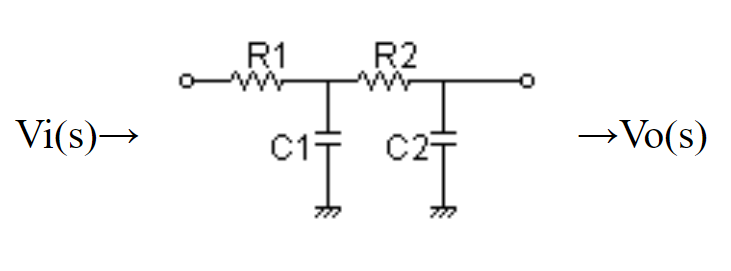
\includegraphics[width=0.5\linewidth]{Hardware/RCfilter}
	\caption{Passivt 2. Ordens lavpasfilter - RC}
	\label{fig:RCfilter}
\end{figure}

Efter beregninger på RC-filteret, se afsnit \vref{RC-filter}, vurderes det, at det er bedre for systemet med et aktivt filter. Vores endelige beslutning omkring filtertype falder derfor på et aktivt 2. ordens lavpasfilter af typen Sallen Key.

\textbf{Sallen Key filter:} 

\begin{figure}[h!]
	\centering
	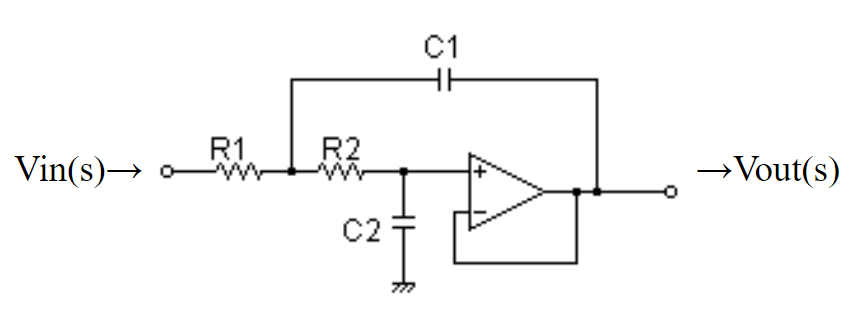
\includegraphics[width=0.5\linewidth]{Hardware/SallenKey}
	\caption{Aktivt 2. Ordens lavpasfilter - Sallen Key}
	\label{fig:SallenKey}
\end{figure}

\clearpage
  
\subsection{Beregninger: RC-filter} \label{RC-filter}
\vspace{0.2 cm}
Overføringsfunktion: 
\[ T(s)=K \cdot \frac{\omega_{0}^{2}}{{s^{2}+2 \cdot \zeta \cdot \omega_{0}\cdot s+\omega_{0}^{2}}} \]

Gain:
\[ K=1 \]



Da vi ikke forstærker signalet yderligere med dette filter sættes $K=1$.
\[ V_{in}=4V \]
\[ V_{out}=4V \]

Frekvens:
\[ \omega_{0}=\frac{1}{\sqrt{R_{1} \cdot R_{2} \cdot C_{1} \cdot C_{2}}} \]

Dæmpningsfaktor:
\[ \zeta= \frac{R_{1} \cdot C_{1} + R_{1} \cdot C_{2}+R_{2} \cdot C_{2}}{2 \cdot \sqrt{R_{1} \cdot R_{2} \cdot C_{1} \cdot C_{2}}} \]

Frekvens og dæmpningsfaktor indsættes nu i overføringsfunktionen:
\[ T(s)=\frac{\frac{1}{R_{1} \cdot R_{2} \cdot C_{1} \cdot C_{2}}}{s^{2}+2 \cdot (\frac{R_{1} \cdot C_{1} + R_{1} \cdot C_{2}+R_{2} \cdot C_{2}}{2 \cdot \sqrt{R_{1} \cdot R_{2} \cdot C_{1} \cdot C_{2}}}) \cdot (\frac{1}{\sqrt{R_{1} \cdot R_{2} \cdot C_{1} \cdot C_{2}}}) \cdot s + (\frac{1}{R_{1} \cdot R_{2} \cdot C_{1} \cdot C_{2}})}  \]

$T(s)$ simplificeres:
\[ T(s)=\frac{1}{s \cdot C_{1} \cdot R_{1} +s \cdot C_{2} \cdot R_{1}+s \cdot C_{2} \cdot R_{2}+s^{2}\cdot C_{1} \cdot C_{2} \cdot R_{1} \cdot R_{2} +1} \]

$T(s)$ simplificeres yderligere:
\[ T(s)=\frac{1}{(R_{1} \cdot C_{1} \cdot s+1) \cdot (R_{2} \cdot C_{2} \cdot s +1) \cdot R_{1} \cdot C_{2} \cdot s} \]

For at gøre beregningen af komponenterne mulig bestemmes $ C_{1} $ og $ C_{2} $ med samme værdi. Værdien er valgt tilfældigt ud fra hvilke komponenter, der findes i laboratoriet:
\[ C_{1} = 220 \cdot 10^{-9} \]
\[ C_{2} = 220 \cdot 10^{-9} \]

Da vi nu har to ligninger med to ubekendte kan vi beregne vores to modstande. Vi ved, at en værdi for dæmpningsfaktoren $\zeta$ på 1.5 vil give os reelle tal, så derfor starter vi med at definere $\zeta$ med denne værdi.

\clearpage
\[ \zeta = 1.5 \]
\[ f_{0} = 50 \]
\[ \omega_{0} = 2 \cdot \pi \cdot f_{0} \]

Med formlerne for $\omega_{0}$ og $\zeta$ på forrige side kan vi nu opstille de to ligninger med to ubekendte som følgende: 
\[ \begin{bmatrix}
R_{1} & R_{2}
\end{bmatrix} = \begin{bmatrix}
\omega_{0}=\frac{1}{\sqrt{R_{1} \cdot R_{2} \cdot C_{1} \cdot C_{2}}} \\ 
\zeta= \frac{R_{1} \cdot C_{1} + R_{1} \cdot C_{2}+R_{2} \cdot C_{2}}{2 \cdot \sqrt{R_{1} \cdot R_{2} \cdot C_{1} \cdot C_{2}}}
\end{bmatrix} \rightarrow \begin{bmatrix}
14468,63 & 14468,63 \\ 7234,32
& 28937,26 
\end{bmatrix}\]

Alle beregninger er udregnet i Mathcad Prime 4.0 og der er her solvet for $R_{1}$ og $R_{2}$.

\begin{figure}[h!]
	\centering
	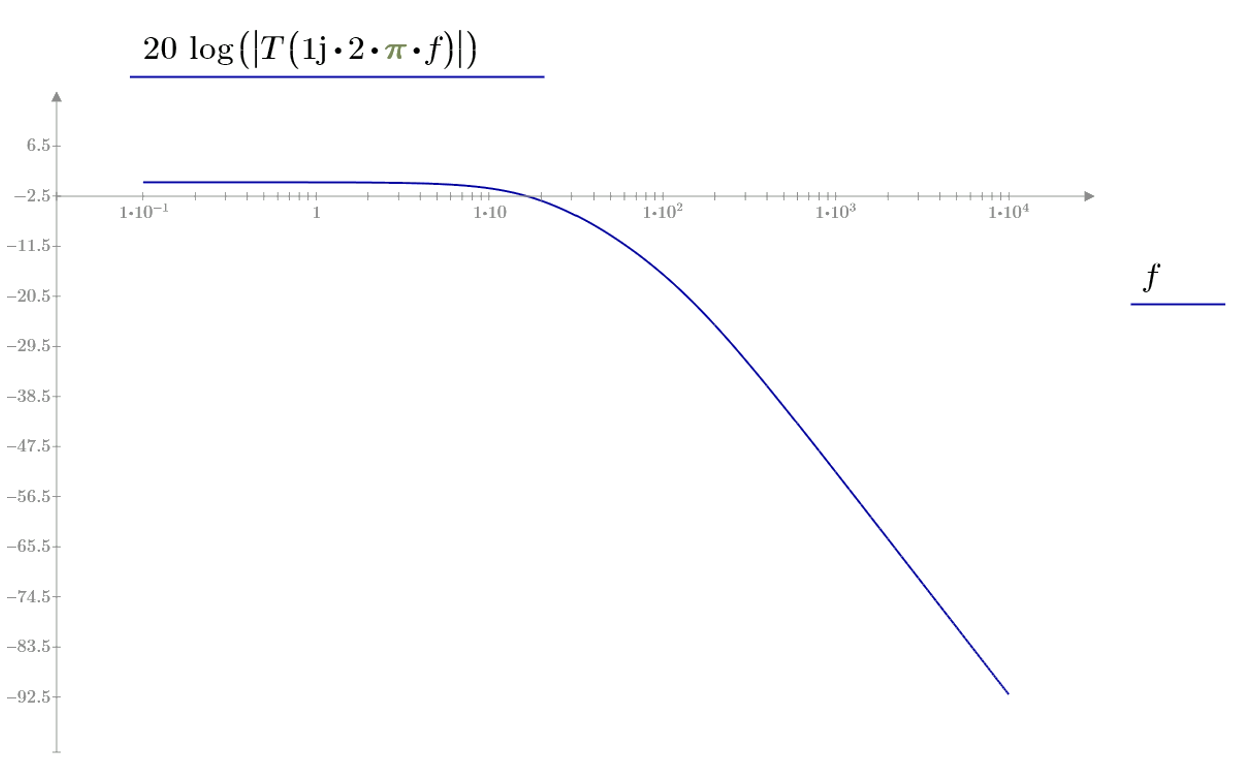
\includegraphics[width=0.7\linewidth]{Hardwaredesign/RCRCfilter1}
	\caption{Bodeplot af RCRC-filter}
	\label{fig:RCRCfilter1}
\end{figure}

\begin{figure}[h!]
	\centering
	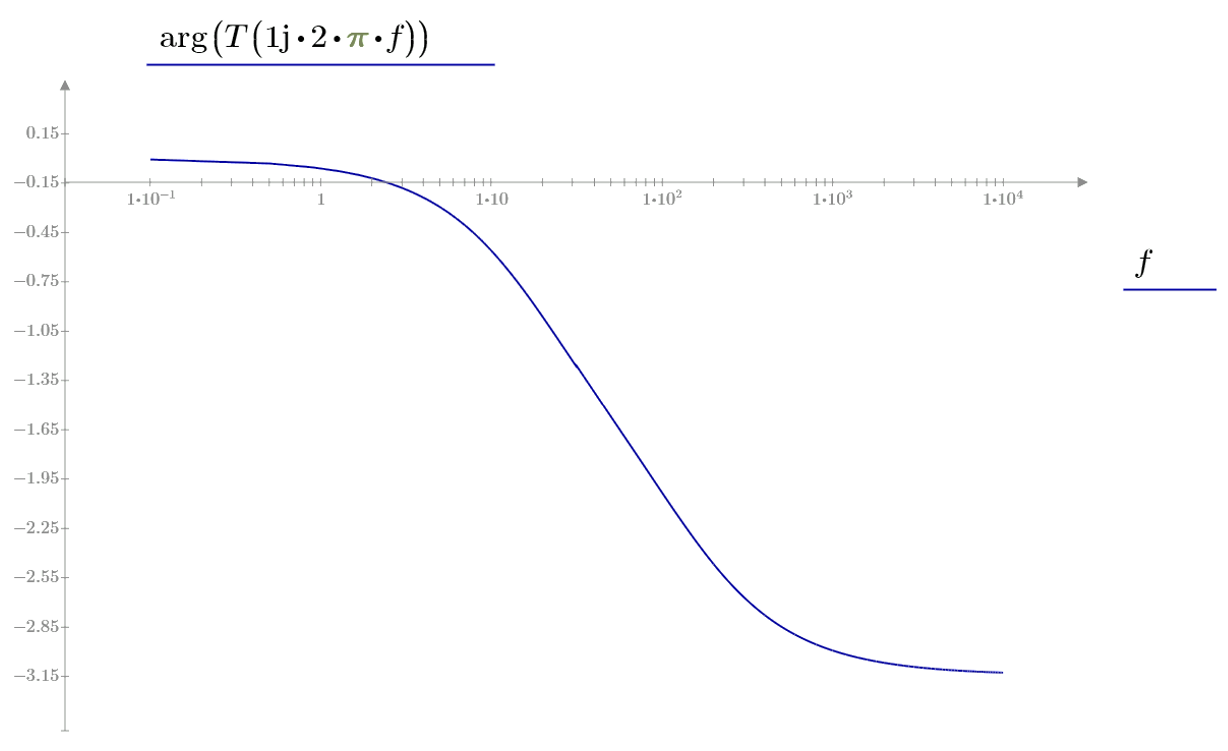
\includegraphics[width=0.7\linewidth]{Hardwaredesign/RCRCfilter2}
	\caption{Plot af RCRC-filter}
	\label{fig:RCRCfilter2}
\end{figure}

\clearpage

For at få en lavere dæmpningsfaktor $ \zeta $ og dermed et fladere bodeplot har vi været nødsaget til at vælge et andet filter. Ændrer vi på værdien på RCRC-filteret vil beregningen af de to modstande ende i komplekse tal, og det er vi ikke interresseret i.  Grundet disse overvejelser er vi kommet frem til, at vælge et aktivt lavpasfilter af typen Sallen Key. Valget er faldet på et aktivt filter frem for et passivt, da vi med et aktivt filter kan stole på en lav udgangsimpedans, der ikke påvirker indgangsimpedansen på AD-converteren. Vi kan med et passivt filter ikke være sikre på en lav udgangsimpedans og ville derfor være nødsaget til at regne på de forskellige komponenter for at få den lavest mulige, der skal være minimum 10 gange mindre end indgangsimpedansen på AD-converteren.

\subsection{Beregninger: Sallen Key filter}
\vspace{0.5 cm}
\[ C_{1} = 680 \cdot 10^{-9} \]
\[ C_{2} = 330 \cdot 10^{-9} \]

Grundet Unity Gain Method kan vi vælge vores to modstande $ R_{1} $ og $ R_{2} $ til at være ens.
\[ R_{1} = 6,71 k\Omega \]
\[ R_{2} = 6,71 k\Omega \]

De valgte komponenter indsættes i nedenstående udtryk for $ \omega_{0} $, så vi derefter kan bestemme vores knækfrekvens $ f_{0} $.
\[ \omega_{0}=\frac{1}{\sqrt{R_{1} \cdot R_{2} \cdot C_{1} \cdot C_{2}}}=314,605 \]

Vi solver for knækfrekvensen $ f_{0} $ på baggrund af de valgte komponenter:
\[ f_{0}:=\omega_{0}=2\cdot \pi \cdot f_{0} \rightarrow 50,07 \]

Vi kan endvidere udregne vores dæmpningsfaktor $ \zeta $, der bestemmes via denne simple formel: 
\[ \zeta=\sqrt{\frac{C_{2}}{C_{1}}}=0,697 \]

Vi er meget tilfredse med denne dæmpningsfaktor, der er noget lavere end den før beregnede dæmpningsfaktor på RC-filteret, der blev beregnet til at skulle være $ \zeta = 1,5 $. Vi plotter filteret i MathCad Prime for at se resultatet af vores dæmpning. Vi får følgende resultat:
\[ T(s)=\frac{\omega_{0}^{2}}{{s^{2}+2 \cdot \zeta \cdot \omega_{0}\cdot s+\omega_{0}^{2}}} \]

\clearpage

\begin{figure}[h!]
	\centering
	\includegraphics[width=0.7\linewidth]{Hardware/Filterplot1}
	\caption{Bodeplot af Sallen Key filteret}
	\label{fig:Filterplot1}
\end{figure}

Vi kan på plottet se, at filteret dæmper med ca 40 $ dB $ pr. dekade, som et 2. ordens filter skal. Vi kan dog samtidig se, at filteret allerede er dæmpet med 3 $ dB $ ved begyndelsen. Dette er konsekvensen af dæmpningsfaktoren, som dog opfører sig noget pænere, end RC-filteret gjorde. 

\begin{figure}[h!]
	\centering
	\includegraphics[width=0.7\linewidth]{Hardware/Filterplot2}
	\caption{Plot af Sallen Key filteret}
	\label{fig:Filterplot2}
\end{figure}

\clearpage

\subsection{Test af filter}
\vspace{0.2 cm}
For at teste filteret har vi brugt Waveforms til at generere et sinussignal med en masse forskellige frekvenser. Vi kan her igen konstatere, at signalet er dæmpes lidt før knækfrekvensen på 50 Hz, ca. med 3 dB som forventet ud fra figur \vref{fig:Filterplot1}. Vi har indsendt signaler med frekvenser mellem 10 Hz og 500 Hz og kan ud fra den udregnede dB se, at signalet dæmpes med de ca 40 dB pr. Dekade som forventes af et 2. ordens filter. I nedenstående tabel \vref{tab:filtertest} ses resultatet af testen af filteret.
\vspace{0.2 cm}
\begin{table}[h!]
	\centering
	\begin{tabular}{l|l|l|l|l}
		\multicolumn{5}{l}{\textbf{Test af filter}} \\
		\hline
		\textbf{Frekvens (Hz)} & \textbf{Amplitude (V)} & \textbf{Offset} & \textbf{Amplitude (V)} & \textbf{dB} \\
		& Input &  & Output & (20*log(Vout/Vin) \\
		\hline
		10 & 2 & 0 & 2 & 0 \\
		\hline
		30 & 2 & 0 & 1,905 & -0,422700313 \\
		\hline
		40 & 2 & 0 & 1,7164 & -1,328229796 \\
		\hline
		50 & 2 & 0 & 1,4416 & -2,843704441 \\
		\hline
		60 & 2 & 0 & 1,1668 & -4,680671504 \\
		\hline
		70 & 2 & 0 & 0,9577 & -6,396010165 \\
		\hline
		80 & 2 & 0 & 0,7546 & -8,466263896 \\
		\hline
		90 & 2 & 0 & 0,6172 & -10,21208157 \\
		\hline
		100 & 2 & 0 & 0,5037 & -11,9771609 \\
		\hline
		110 & 2 & 0 & 0,432 & -13,31092498 \\
		\hline
		120 & 2 & 0 & 0,3603 & -14,88731467 \\
		\hline
		130 & 2 & 0 & 0,3066 & -16,2891569 \\
		\hline
		140 & 2 & 0 & 0,2707 & -17,3708348 \\
		\hline
		150 & 2 & 0 & 0,2286 & -18,83907539 \\
		\hline
		170 & 2 & 0 & 0,1772 & -21,05132556 \\
		\hline
		190 & 2 & 0 & 0,1438 & -22,86542219 \\
		\hline
		210 & 2 & 0 & 0,1163 & -24,70900562 \\
		\hline
		250 & 2 & 0 & 0,084 & -27,53501419 \\
		\hline
		290 & 2 & 0 & 0,0613 & -30,27139042 \\
		\hline
		330 & 2 & 0 & 0,0467 & -32,6342623 \\
		\hline
		370 & 2 & 0 & 0,0374 & -34,56316787 \\
		\hline
		410 & 2 & 0 & 0,0299 & -36,50717615 \\
		\hline
		450 & 2 & 0 & 0,0247 & -38,16666085 \\
		\hline
		500 & 2 & 0 & 0,0201 & -39,95667876
	\end{tabular}
\caption{Test af Sallen Key filter}
\label{tab:filtertest}
\end{table}

\clearpage
Her ses et par eksempler på nogle af de sinussignaler, der blev sendt ind vha. Waveforms. Hér ses det hvordan signalet er dæmpet mere og mere ved højere frekvenser og derfor får en lavere amplitude.

10 Hz:
\begin{figure}[h!]
	\centering
	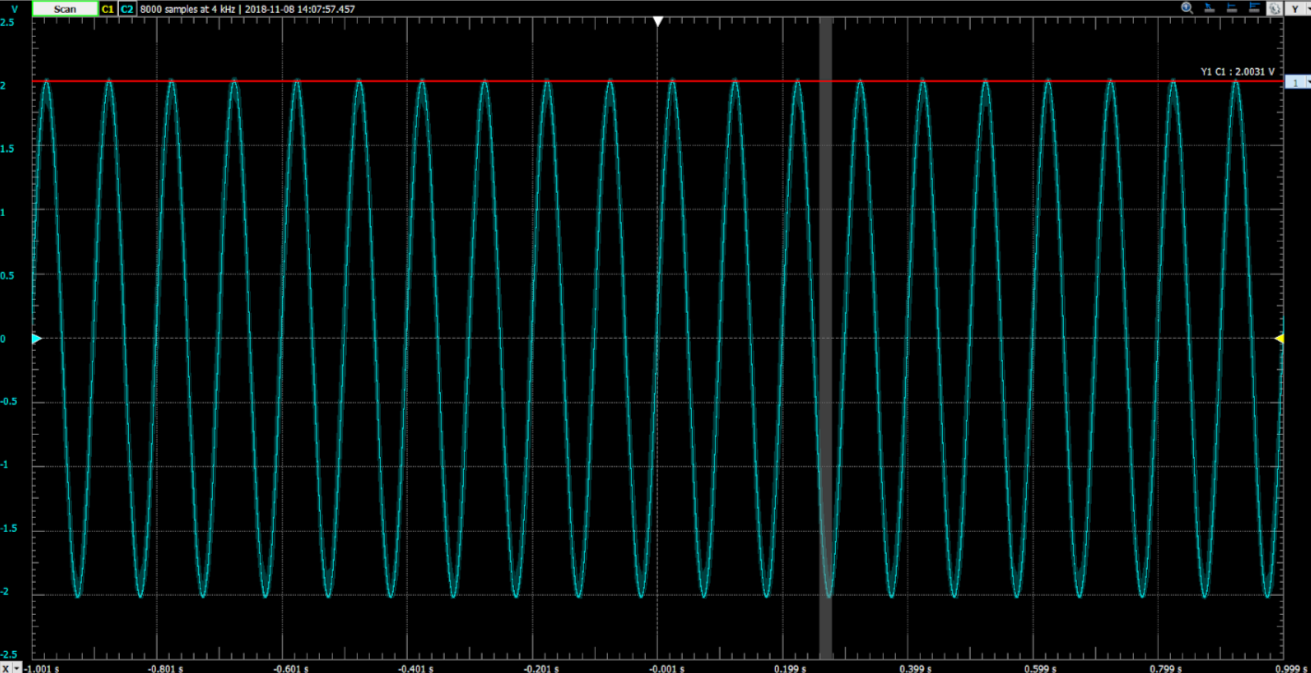
\includegraphics[width=1\linewidth]{Hardwaredesign/10hz}
	\caption{Test af filter: 10 Hz}
	\label{fig:10hz}
\end{figure}

50 Hz: 
\begin{figure}[h!]
	\centering
	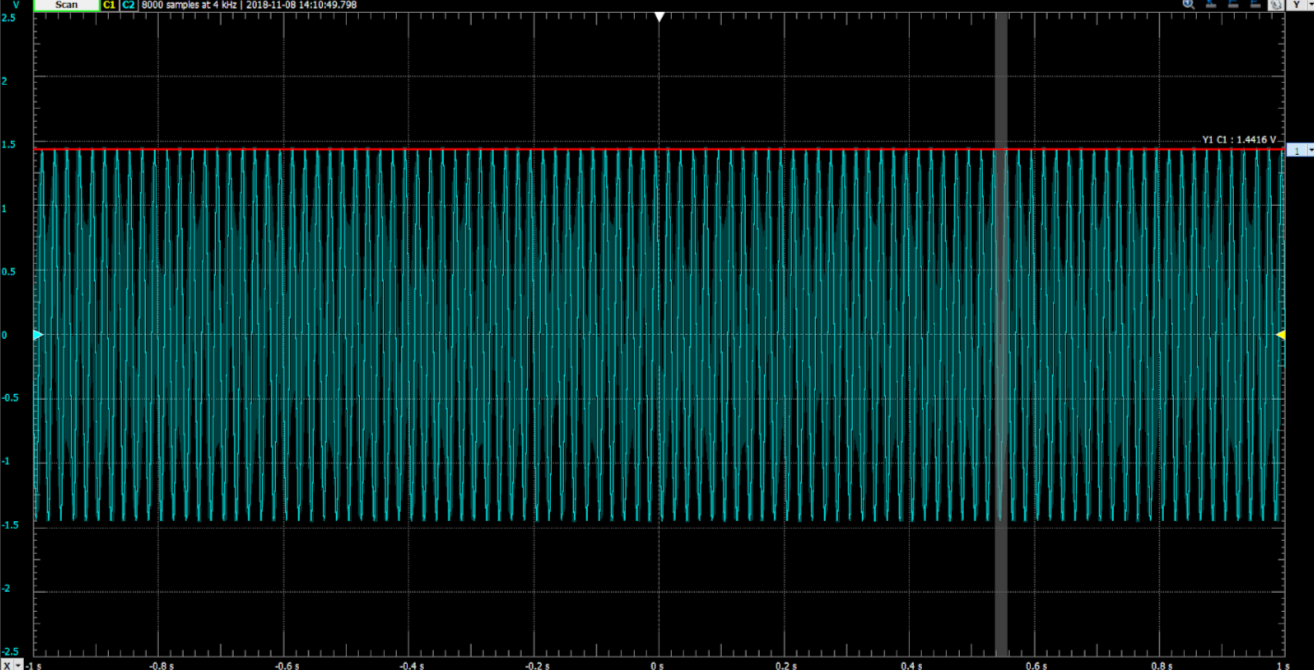
\includegraphics[width=1\linewidth]{Hardwaredesign/50hz}
	\caption{Test af filter: 50 Hz}
	\label{fig:50hz}
\end{figure}
\clearpage
100 Hz:
\begin{figure}[h!]
	\centering
	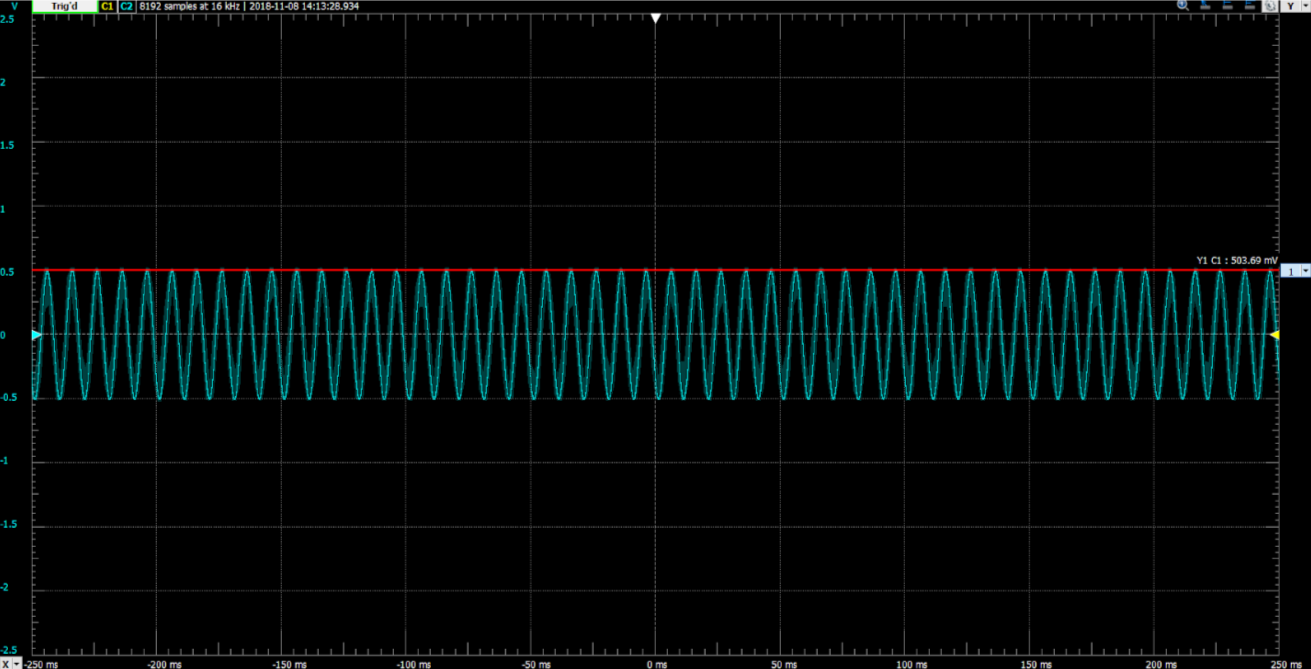
\includegraphics[width=1\linewidth]{Hardwaredesign/100hz}
	\caption{Test af filter: 100 Hz}
	\label{fig:100hz}
\end{figure}

250 Hz:
\begin{figure}[h!]
	\centering
	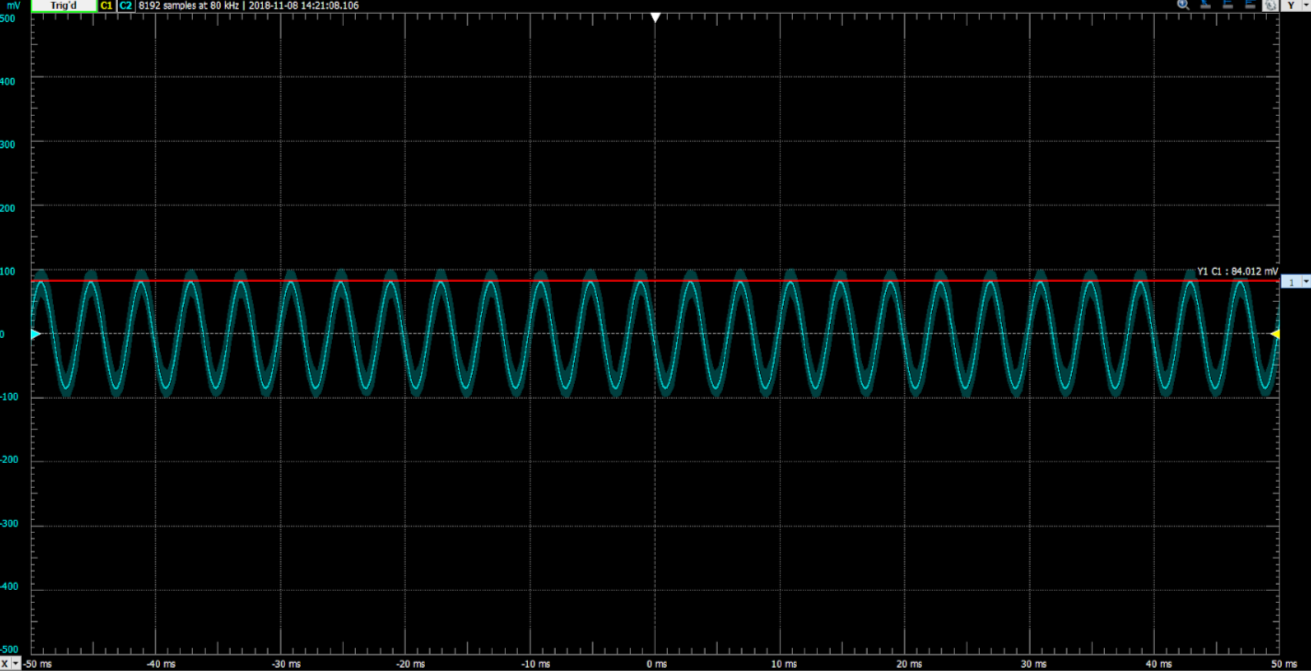
\includegraphics[width=1\linewidth]{Hardwaredesign/250hz}
	\caption{Test af filter: 250 Hz}
	\label{fig:250hz}
\end{figure}
\clearpage
500 Hz:
\begin{figure}[h!]
	\centering
	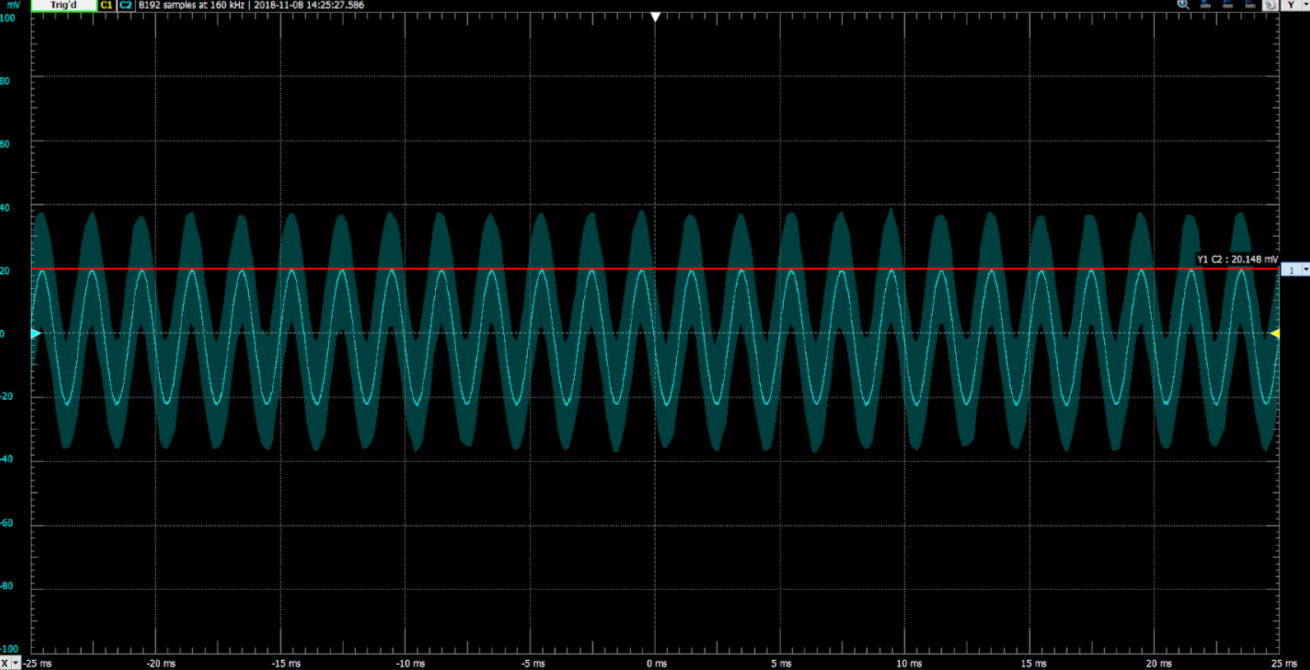
\includegraphics[width=1\linewidth]{Hardwaredesign/500hz}
	\caption{Test af filter: 500 Hz}
	\label{fig:500hz}
\end{figure}

